At the physical level, computer memory consists of a large number of
flip flops.
Each flip flop consists of a few transistors,
and is capable of storing one bit.
Individual flip flops are addressable by a unique identifier,
so we can read and overwrite them. 
Thus, conceptually, we can think of all of our computer's memory as
just one giant array of bits that we can read and write.

Since as humans, we are not that good at doing all of our thinking and
arithmetic in bits, we group them into larger groups,
which together can be used to represent numbers.
8 bits are called 1 byte; beyond bytes, there are words
(which are sometimes 16, sometimes 32 bits).
Thus, more often, we conceptually regard our computer's memory as one
large (size $2^{32}$ or so) array of bytes.
A lot of things are stored in this memory.

\begin{enumerate}
\item All variables and other data used by all programs.
\item But also the code of all programs, including the code for the
  operating system.
\end{enumerate}

The compiler and the operating system work together to take care of
most memory management for you, but it is instructive to see what is
going on under the hood.

When you compile your code, the compiler can examine primitive data
types and calculate how much memory they will need ahead of time.
The required amount is then allocated to the program in the
\todef{stack}\footnote{This space is called the stack space because as
  functions get called, their memory gets added on top of existing
  memory. As they terminate, they are removed in a LIFO (last in,
  first out) order. We will encounter this concept in more detail in
  Chapter~\ref{chap:stacksqueues}, when we learn about the Stack data type.}
space. For example, consider the following declarations: 
\begin{verbatim}
int n;
int x[10];
double m;
\end{verbatim}
The compiler can immediately see that the code requires
$4+4\times10+8=52$ bytes\footnote{That's with the current sizes for
  integers and doubles. About 20 years ago, \code{int} were typically
  2 bytes, and \code{double} 4 bytes. Your code should never have to
  depend on what is at this moment the size of the basic data types.}.

It will insert code that will interact with the operating system to
request the necessary number of bytes on the stack for your variables
to be stored. In the example above, the compiler knows that the memory
will look as follows:

\begin{figure}[htb]
\setlength{\unitlength}{0.1in}
\begin{picture}(60,8)
\linethickness{0.02mm}
\multiput(0,1)(1,0){55}{\line(0,1){4}}
\put(0,1){\line(1,0){60}}
\put(0,5){\line(1,0){60}}
\linethickness{0.5mm}
\put(0,1){\line(0,1){4}}
\put(4,1){\line(0,1){4}}
\put(44,1){\line(0,1){4}}
\put(52,1){\line(0,1){4}}

\put(0.5,6){\line(1,0){3}}
\put(0.5,6){\line(0,-1){0.5}}
\put(3.5,6){\line(0,-1){0.5}}
\put(2,7){$n$}
\put(4.5,6){\line(1,0){3}}
\put(4.5,6){\line(0,-1){0.5}}
\put(7.5,6){\line(0,-1){0.5}}
\put(5,7){$x[0]$}
\put(24.5,6){\line(1,0){3}}
\put(24.5,6){\line(0,-1){0.5}}
\put(27.5,6){\line(0,-1){0.5}}
\put(25,7){$x[5]$}
\put(44.5,6){\line(1,0){7}}
\put(44.5,6){\line(0,-1){0.5}}
\put(51.5,6){\line(0,-1){0.5}}
\put(48,7){$m$}
\end{picture}
\caption{The layout of memory on the stack for the declaration above.}
\end{figure}

It knows the exact memory address of each variable;
in fact, whenever we write \code{n}, this gets translated into
something like ``memory address 4127963'' internally.

Notice that if we attempted to access $x[10]$ here, we would access
the data associated with $m$, and may end up reading (or overwriting)
some of its bits.
This would almost certainly have very undesirable consequences for the
rest of the program.
In fact, accessing out-of-bounds memory locations is the root cause of
a huge fraction of software bugs,
ranging from CSCI 104 homework nightmares
to professional software glitches that cause billions of dollars in
damages and massive security breaches.

\begin{figure}[htb]
\centering
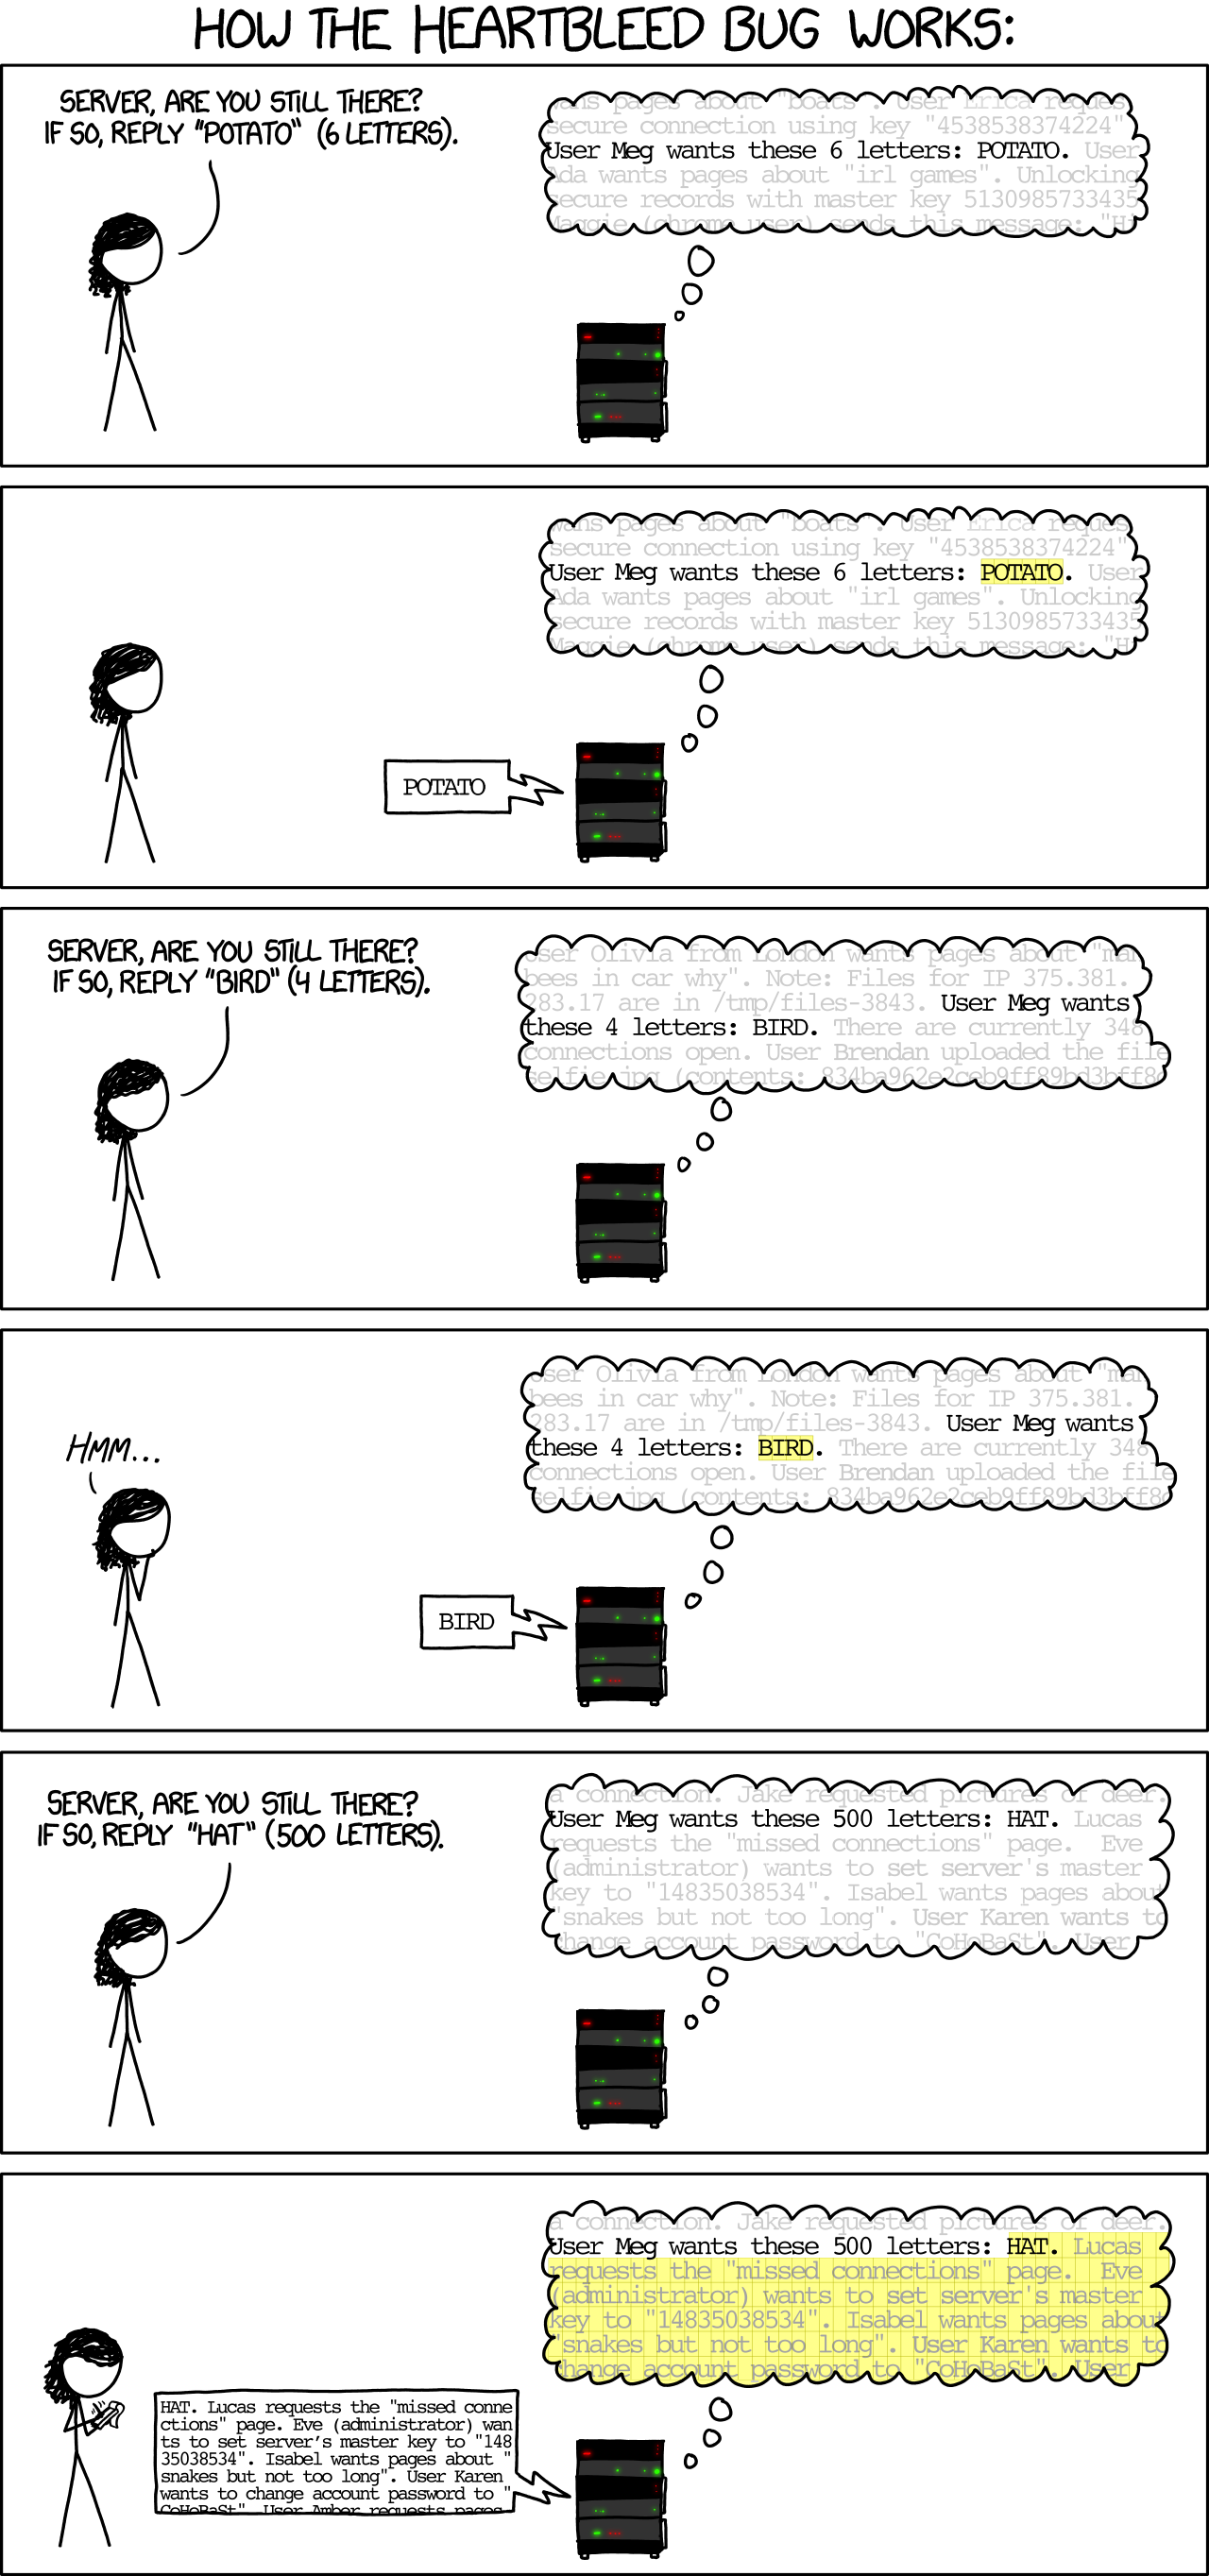
\includegraphics[scale=0.4]{comics/xkcd_heartbleed_explanation.eps}
\caption{XKCD \# 1353: Explanation of the Heartbleed Bug}
\end{figure}

When functions call other functions, each function gets its own chunk
of stack memory at the moment it is called;
it keeps all its local variables there, but also a program counter
that remembers where in its execution it was.
When the function finishes, its stack memory block is made available
for other purposes again.
For statically allocated variables,
the compiler can take care of all of this, and you typically don't
have to think about it.

\section{Scoping of Variables}
While we are talking about local variables and the stack, we should
briefly talk about the scope of a variable.
Global variables are, of course, accessible to any function or any
block of code in your program.
Local variables in functions or code blocks only exist while the
execution is in the function or the code block.
Local variables are typically stored on the stack.
As soon as the function or block terminates,
the variable is deallocated. 

When the execution of a function is temporarily suspended,
for instance because another function got called inside this one,
the variables are stored on the stack, but not active,
so they cannot be accessed.
Consider the following example:

\begin{verbatim}
void foo (int x)
{
  int y; 
  // do some stuff
}

void bar (int n)
{ 
  int m;
  foo (n+m);
  // do more stuff
}
\end{verbatim}

Here, when \code{bar} calls \code{foo}, the function \code{foo} cannot
access the variables \code{n} or \code{m}.
As soon as \code{foo} finishes, the variables \code{x} and \code{y}
are deallocated, and permanently lost.
\code{bar} now resumes and has access to \code{n} and \code{m},
but not to \code{x} or \code{y}.

You will sometimes have multiple variables (in different parts of your
code) sharing the same name.
For instance, you may have both a global variable \code{n} and a local
variable called \code{n} in a function.
Or you could have code like the following:

\begin{verbatim}
void foo (int n)
{
  int m = 10;
  // do something
  for (int i = 0; i < m; i ++)
    {
      int n = 3, m = 5;
      // do something
      cout << n << m;
    }
}
\end{verbatim}

Here, the \code{cout << n << m} statement would output the innermost
versions, so the values 3 and 5.
As a general rule, when there are multiple variables with the same name,
any reference is to the one in the smallest code block enclosing the
statement that contains that variable.
Of course, as another general rule, when you can, you should avoid
writing code that makes you and others think for a while to figure out
which variable is being referenced with a particular name.

\section{Dynamic allocation}
Static allocation works easily when the compiler can tell at compile
time how much memory will be needed.
However, in many cases, it is not known at compile time how much
memory a program (or particular structure within a program) needs.
As an example suppose that you want to do something like the following:

\begin{verbatim}
int n;
cin>>n;
// create an array a of n integers
\end{verbatim}

Here, at compile time, the compiler does not know how much memory the
array will need. It can therefore not allocate room for a variable on
the stack\footnote{Technically, this is not quite true. Some modern
  compilers let you define arrays even of dynamic sizes, but we advise
  against using this functionality, and instead do things as we write
  in these notes.}.
Instead, the program will need to explicitly ask the operating system
for the right amount of space at run-time. 
This memory is assigned from the \todef{heap}\footnote{This is called
  the heap space since it can be selected from any portion of the
  space that has not been allocated already. While the stack remains
  nicely organized, memory in the heap tends to be more messy and all
  over the place. Hence the name.} space. 

The difference between static and dynamic memory allocation is
summarized in the following table.
To fully understand how dynamic memory allocation works,
we need to spend some time on pointers.

\begin{table}[h]
	\centering
    \begin{tabular}{l|l}
       \textbf{Static allocation}         & \textbf{Dynamic allocation}                \\ \hline
        Size must be known at compile time & Size may be unknown at compile time \\
        Performed at compile time & Performed at run time             \\ 
        Assigned to the stack     & Assigned to the heap              \\ 
        First in last out         & No particular order of assignment \\
        Compiler takes care of deallocation & You must take care of
                                              deallocation \\
    \end{tabular}
\caption{Differences between statically and dynamically allocated memory.}
\end{table}

\section{Pointers}
A pointer is an ``integer'' that points to a location in memory ---
specifically, it is an address of a byte\footnote{This means that all
pointers are of the same size, and that the size of a pointer used by
a computer places a limit on the size of memory it can address.
For example, a computer using typical 32-bit pointers can only use up to
$2^{32}$ bytes or $4$ gigabytes of memory.
The modern shift to 64-bit architectures turns this to $2^{64}$ bytes,
which will be enough for a while.}. 

In C/C++, pointer types are declared by placing a star `*' behind a
regular type name.
Thus, \code{int *p; char *q; int **b; void *v;} all declare pointers.
In principle, all of these are just addresses of some memory location,
and C/C++ does not care what is stored at the address.
Declaring them with a type (such as \code{int}) is mostly for the
programmer's benefit:
it often prevents you from messing up the use of the
data stored in the location.
It also affects the way some arithmetic on memory locations is done,
which we will see below.

Two of the ways in which ``regular'' variables and pointers often
interact are the following:
\begin{enumerate}
\item You want to find out where in memory a variable resides, i.e.,
  get the pointer to that variable's location.
\item You want to treat the location a pointer points to as a variable,
  i.e., access the data at that location, by reading it or overwriting
  it.
\end{enumerate}
The following piece of code illustrates some of these, as well as
pitfalls one might run into.

\begin{verbatim}
int* p = nullptr, *q;	//Pointers to two integers
int i, j;
i = 5; j = 10;
p = &i;	  //Obtain the address of i and save it to p
cout << p;  //Prints the value of p (address of i)
cout << *p; //Prints the value of the integer that p points to (which is the value of i)
*p = j;   // Overwrites the value of the location that p points to (so, i) with the value of j
*q = *p;  // Overwrites the value of the location that q points to with the one that p points to
q = p;    // Overwrites the pointer p with q, so they now point to the same location
\end{verbatim}

A few things are worth noting here.
\begin{enumerate}
\item The last two commands both result in \code{*p} being equal to
\code{*q}, but in different ways. In the first case, we copy the
\emph{value} from one location to the other, while in the second, 
we make both point to the same place.
This will manifest itself later: if you make a change to \code{*p}
after writing \code{q = p}, it will also change \code{*q};
this does not happen if you wrote \code{*q = *p}.
\item In our code example, the second-to-last command is very risky,
  and will likely cause a run-time error.
  The piece of code did not initialize \code{q},
  so it points to an arbitrary memory location, quite possibly location 0.
  The code is trying to overwrite this location,
  which most likely the program is not allowed to do.
  The location may belong to the operating system or
  some other program\footnote{Fortunately, nowadays, all that happens
    is that your program throws a run-time error. In the past, the OS
    would often allow you to do such an overwrite, in which case often
    some complete system crashes would happen.}.
\item \code{nullptr}\footnote{\code{nullptr} was introduced in
    C++11. You will need to use the C++11 flag in order to be able to
    use this keyword. In older versions, the keyword used was
    \code{NULL}, which still works in later versions.} is a special
  pointer, typically used to express that a pointer is ``not pointing
  anywhere.'' Of course, it is actually pointing somewhere.
  \code{nullptr} is basically just another name for the number 0.
  But since your code should never access memory location 0,
  having this as a ``not initialized'' value is a useful convention.
\item Our earlier comment about the perils of
  uninitialized pointers suggests that whenever you have a pointer
  variable, you always assign it \code{nullptr} right away as you declare
  it. In our example, we did that for \code{p}, but should also have
  done the same for \code{q}.
  That way, if you later forget to assign it a memory location before
  dereferencing it, at least, it will cause a crash of your program,
  rather than possibly processing some garbage that it reads from the
  location.
  This is good coding practice to reduce your debug time.
\item \code{\&} and \code{*} are \emph{inverses} of each other.
  Thus, \code{\&*p} and \code{*\&p} are the same as \code{p}.
  (The exception is that \code{\&*p} throws a runtime error when applied
  to \code{p==nullptr}, instead of being equal to \code{p}.)
\end{enumerate}

In general, it is quite easy to mess up with pointers.
A few rules of thumb will weed out common mistakes,
but generally speaking, even experienced programmers produce runtime
errors frequently when dealing with pointers.

\begin{figure}[htb]
\centering
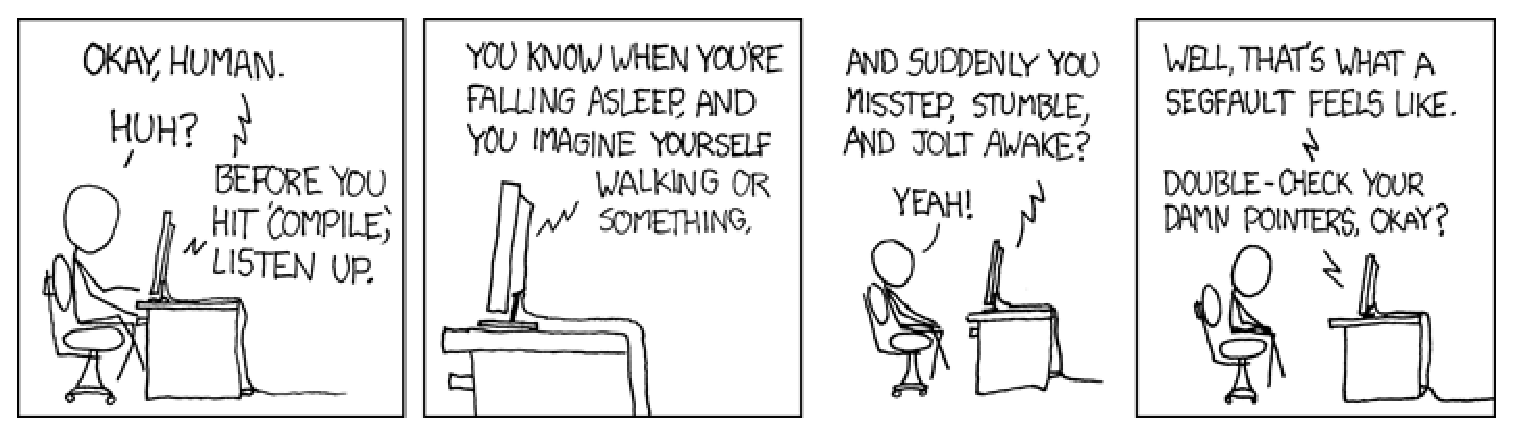
\includegraphics[scale=0.6]{comics/xkcd_compiler_complaint.eps}
\caption{XKCD \# 371: Check your Pointers!}
\end{figure}


We discussed before that pointers are basically just integers.
They differ in that arithmetic is somewhat different.
When you have a pointer \code{p} to an \code{int},
and you write \code{p+1},
the compiler assumes that what you want is the address
where the next \emph{integer} will start, which is 4 bytes later.
Thus, the actual address referenced by writing \code{p+1} is actually
4 bytes after the address of \code{p}.

This is where the type of pointer matters, as we mentioned above. 
When you have a \code{void*}, then addition really does refer to
adding individual bytes. For all other pointer types, when you write
\code{p+k} for a pointer \code{p} and integer \code{k}, 
this references memory location \code{p+k*size(<type>)}, where
\code{<type>} is the type of the pointer \code{p}.

\section{Dynamic Memory Allocation}
In order to dynamically allocate and deallocate memory,
C++ uses the functions \code{new} and \code{delete}.
They are built on the C functions \code{malloc} and \code{free},
which you can read about in Section~\ref{sec:dynamic-memory:malloc-free}.
The C++ versions shield you from some of the internals and will help
you avoid common mistakes in dealing with dynamic memory.

\subsection{C++ Style}
In C++, you allocate dynamic memory with \code{new()}
and deallocate it with \code{delete()}.
Let us look at allocation of memory first.
To solve our small problem from earlier --- ask the user for an array
size and allocated that much memory --- we would write the following:

\begin{verbatim}
int n;
int *b;
cin >> n;
b = new int[n];
for (int i=0; i<n; i++)
    cin >> b[i];
\end{verbatim}
The desired number of \code{int} spaces in the array is given in
square brackets, as with statically allocated arrays.

If we wanted space for just one integer, we could write
\code{int *p = new int;}
While this is not really very useful for a single integer,
it will become very central to allocating objects later,
where we often allocate one at a time dynamically.

When you allocate a single object, you can optionally give it a
default value in parentheses, as follows:
\code{int *p = new int (42); }
This code dynamically allocates a pointer to an integer,
and initializes the memory location's value to 42.
We will see later (in Sections~\ref{sec:classes:constructors} and
\ref{sec:overloading:copy-constructors}) that this is a special case
of copy constructors.

Another thing to observe here is that we can reference \code{b} just
like an array, and we write \code{b[i]}.
The compiler treats this exactly as \code{*(b+i)}, and, as you
probably remember from the part about pointer arithmetic, this points
to the \Kth{i} entry of the array.
In fact, that's exactly how C/C++ internally treats all arrays anyway;
basically, they are just pointers.

If we wanted to write \code{b[i]} in a complicated way by doing all
the pointer arithmetic by hand, we could write instead
\code{*((int*) ((void*) b + i * sizeof(int)))}.
Obviously, this is not what we like to type (or have to understand),
but if you understand everything that happens here, you are probably
set with your knowledge of pointer arithmetic and casting.

\smallskip

To release memory, we use the \code{delete} operator, as follows:
\begin{verbatim}
delete [] b;
delete p;
\end{verbatim}
The first example deallocates an array,
while the second deallocates a single instance of a variable
(a single \code{int} in our earlier example).
``Deallocating'' means that your code tells the operating system that
it won't need the memory at \code{p} any more, and the operating
system should feel free to reuse it for other purposes.

Note that \code{delete} does nothing to the pointers \code{b} or
\code{p} themselves;
it only deallocates the memory that they pointed to.
Thus, it is very good programming practice to immediately set the
pointer to \code{nullptr} after deallocating the memory it points to;
this way, your code will not attempt to tamper with invalid memory.

What could happen otherwise is the following:
you returned the memory to the operating system, which used it for
another variable (in your program or maybe another program).
Now you may accidentally overwrite or read the value that was written
into this new variable. Such a bug will be very hard to diagnose.
If you instead set the pointer to \code{nullptr}, you will instead get
a runtime error when you try to access the memory,
which is typically much easier to pin down and debug.

\subsection{C Style Memory Allocation (*)} \label{sec:dynamic-memory:malloc-free}
While we use C++ in this class, it is useful to understand the C-style
memory allocation as well.
After all, the C++ functions are built on top of the C ones,
and the C style is closer to the machine level, providing you perhaps
with a better understanding of what goes on inside your machine.

To allocate memory in C, one uses the function
\code{void* malloc (unsigned int size)}.
This function requests \code{size} bytes of memory from the operating
system, and returns the pointer to that location as a result. 
If for some reason, the OS failed to allocate the memory
(e.g., there was not enough memory available),
\code{nullptr} is returned instead.

The main difference between \code{malloc} and \code{new},
besides small syntax issues (square brackets for \code{new}
vs.~parentheses for \code{malloc}), is that when using \code{malloc},
you have to specify the number of \emph{bytes} you would like,
whereas with \code{new}, you specify the number of \emph{items} in
your array. 
This means that we need a way to figure out how many bytes will be
required for the number of items we want.
The way to find this out is the \code{sizeof} function.
When you write \code{sizeof (t)}, it returns the number of bytes for
each item of type \code{t};
for instance, \code{sizeof (int)} will give you the number of bytes in
an integer.
Even if you think that you know how many bytes a type will need,
you should never hard-code that constant, as it may change over time.
Even if right now, on your current computer, an integer needs 4 bytes,
that may not be the case forever if you reuse your code later.

Another difference between \code{malloc} and \code{new} is that
\code{malloc} returns a \code{void*},
since it does not know what kind of data we want to store at the
location.
As a result, we have to cast the pointer to the type that we want in
the end, for instance, an \code{int *}.
Taken together, the code we had earlier is therefore written as:

\begin{verbatim}
int n;
int* b;
cin >> n;
b = (int*) malloc(n * sizeof(int));
\end{verbatim}

For good coding practice, we should probably also check whether
\code{b==nullptr} before dereferencing it,
but this example is supposed to remain short.

\smallskip

The analogue to \code{delete} in C++ is the function 
\code{void free (void* pointer)};
it releases the memory located at \code{pointer} for reusing.
So our earlier code for releasing memory would now become

\begin{verbatim}
free (b);
free (p);
\end{verbatim}

Just like \code{delete}, the function \code{free} does not change the
pointer (\code{b} or \code{p}) and only deallocates the memory.
So as with \code{delete}, it is good coding practice to set the
pointers to \code{nullptr} (or, in C, \code{NULL}) after they are
deallocated.


\section{Memory Leaks}
Let us look a little more at the things that can go wrong with dynamic
memory allocation.

\begin{verbatim}
double *x;
...
x = new double [100];
...
x = new double [200]; // We're gonna need a bigger array!
...
delete [] x;
\end{verbatim}

This code will compile just fine, and most likely will not crash,
at least not right away.
We correctly allocate an array of 100 \code{double},
use it for some computation,
and then allocate an array of 200 \code{double} when we
realize that we need more memory.

But notice what happens here.
The moment we do the second allocation, \code{x} gets overwritten with
a pointer to the newly allocated memory block.
At that point, we have no more recollection of the pointer to
the previous memory block.
That means we cannot read it, write it, or deallocate it.
When at the end of the code snippet,
the program calls \code{delete [] x},
it successfully deallocates the second allocated block,
but we are unable to tell the operating system that we do not need the
first block any more. 
Thus, those 800 bytes will never become available again
(until our program terminates --- but for all we know, it may run for
several years as a backend server somewhere).

This kind of situation is called a \todef{memory leak}:
available memory is slowly leaking out of the system.
If it goes on long enough, our program may run out of memory and crash
for that reason. It could be quite hard to diagnose why the crash
happened if it does after a long time of running.

It is good practice to keep close track of the memory blocks you
reserve, and make sure to \code{delete} (or \code{free}) memory
pointed to by a pointer before reusing the pointer\footnote{There are tools
for checking your code for memory leaks, and we recommend
familiarizing yourself with them. The most well-known one, for which
the course web page contains some links, is called \code{valgrind}.}.
A better version of the code above would be the following:

\begin{verbatim}
double *x;
...
x = new double [100];
...
delete [] x;
x = nullptr;
x = new double [200];
...
delete [] x;
x = nullptr;
\end{verbatim}

That way, the memory gets released while we still have a pointer to
it.
You will recall that it is always good practice to immediately set
pointers to \code{nullptr} after deallocating their memory.
In the middle of the code, that may seem very redundant:
after all, the example program immediately overwrites \code{x} with
another value. 
And in fact, here, it \emph{is} completely redundant.
However, we still recommend that you add the line;
for example, you may later insert some code between \code{delete [] x}
and \code{x = new double [200]}, and you might easily insert mistakes there.
And if you are worried about your program wasting time with
unnecessary assignments, don't be --- the compiler will almost certainly
optimize that assignment away anyway, and the final compiled code will look
exactly the same.

One question you may be wondering about is if we could just free the
memory by setting \code{x = nullptr;}
without calling \code{delete [] x} first.
That would only overwrite the pointer, but it would not tell the
operating system that it can have the memory back.
In other words, it would exactly \emph{create} a memory leak.
Whenever you want to return memory to the system, you must do so
explicitly\footnote{There are other programming languages that do much
  more of the garbage collection and memory handling for you,
  but C/C++ is not one of them.}. 

As a side note, if you look up some of this information online or in
other sources, keep in mind that the pool of memory where you allocate
variables with \code{new} (or \code{malloc}) is called the
\todef{memory heap}.
This is different from a data structure known as the \emph{heap} which
you will learn about in Chapter~\ref{chap:priority-queues}.
Unfortunately, people (including us $\ldots$) are not quite consistent
in naming these.
